\documentclass{prova}

\usepackage{amsmath}
\usepackage{amsfonts}

\setlength{\textheight}{25cm}

\renewcommand{\sin}{\,\mbox{sen}\,}
\newcommand{\ds}{\displaystyle}

\professor{Prof.\@ Adriano Barbosa}
\disciplina{C\'alculo Diferencial e Integral II}
\avaliacao{Final}
\curso{Engenharia de Produ\c{c}\~ao}
\data{06/12/2021}

\begin{document}
	\cabecalho{5}  % o numero 5 indica a qnt de quadros na tabela de nota

    \textbf{Todas as respostas devem ser justificadas.}

    \begin{questionario}
        \q{(3 pts) Calcule a \'area da regi\~ao delimitada pelas fun\c{c}\~oes
        $f(x)=\ds\frac{2}{2+\sqrt{x}}$ e $g(x)=\ds\frac{2}{2-\sqrt{x}}$ e pela
        reta $x=1$.}
        \begin{figure}[h]
            \centering
            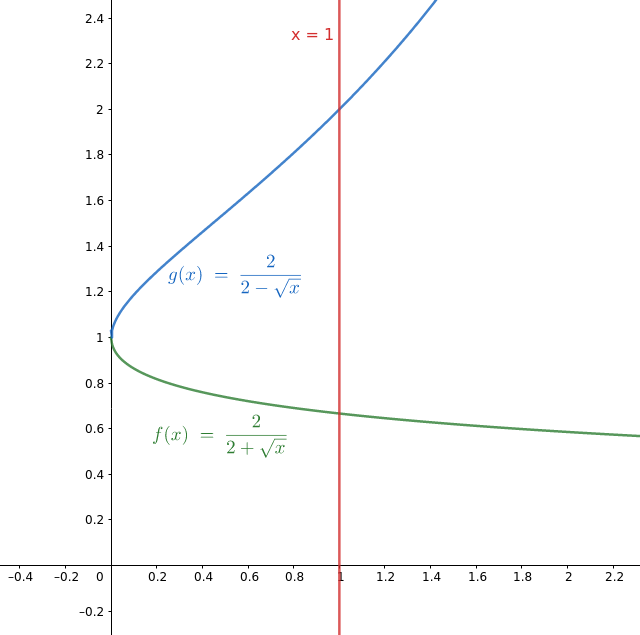
\includegraphics[width=0.5\textwidth]{q1.png}
        \end{figure}
        \q{(2 pts) Determine se as afirma\c{c}\~oes abaixo s\~ao verdadeiras ou falsas
        justificando sua resposta.}
            \begin{questionario}
                \qq{A equa\c{c}\~ao $y'=x+y$ n\~ao \'e linear.}
                \qq{A equa\c{c}\~ao $y'=2y+x+2xy+1$ \'e separ\'avel.}
                \qq{A equa\c{c}\~ao $2^xy'=y$ \'e linear.}
                \qq{A equa\c{c}\~ao $y'+xy=\cos{y}$ \'e linear.}
            \end{questionario}
        \q{(2 pts) Sejam $I=\ds\left(\frac{1}{2}, \infty\right)$ e
        $f:I\rightarrow\mathbb{R}$, $\ds f(x)=e^{x^2}$. Encontre a fun\c{c}\~ao
        $g:I\rightarrow\mathbb{R}$ tal que $f'g' = f'g+fg'$.}
        \q{(3 pts) Encontre a soma da s\'erie cujos termos s\~ao da forma
        $\ds\frac{1}{n}$, onde os \'unicos fatores primos de $n$ s\~ao 3 e 5:}
            \[1+\frac{1}{3}+\frac{1}{5}+\frac{1}{9}+\frac{1}{15}+
            \frac{1}{25}+\frac{1}{27}+\frac{1}{45}+\frac{1}{75}+\cdots\]
    \end{questionario}
\end{document}
